\subsection{Dynamical Systems and Eigenvectors}

In general, a discrete dynamical system can be modeled as:

\[\boxed{\tb{x}(t+1)=A\tb{x}(t)}\]

where the transformation undergone by the system is $\tb{x}(t)\rightarrow\tb{x}(t+1)$ with matrix $A$.
Additionally, note that $\tb{x}(t)=\begin{bmatrix}c(t)\\r(t)\end{bmatrix}$ where $c(t)$ and $r(t)$ are some closed formulas.

Finding $\tb{x}(t)$ for an arbitrary integer $t>0$:

\[\boxed{\tb{x}(t)=A^t\tb{x}(0)=A^t\tb{x}_0}\]

Repeat definition of eigenvector from below:

\begin{framed}
    If $A$ is an $n\times n$ matrix, an eigenvector of $A$ is a nonzero vector $\tb{v}$
    that has the property that $\tb{v}$ and $A\tb{v}$ are parallel.
    Same as saying that $A\tb{v}=\lambda\tb{v}$, so $\lambda$ is an eigenvalue.
\end{framed}

\subsection{Dynamical Systems Example}

Following equations model transformation from $t$ to $t+1$:

\[\boxed{
    \begin{array}{l}
        c(t+1)=0.86 c(t)+0.08 r(t) \\
        r(t+1)=-0.12 c(t)+1.14 r(t)
        \end{array}
}\]

Is discrete dynamical linear system: changed over discrete time interval and dynamic as
variables change according to $t$. As a matrix-vector equation:

\[\left(\begin{array}{cc}
    0.86 & 0.08 \\
    -0.12 & 1.14
    \end{array}\right)\left(\begin{array}{l}
    c(t) \\
    r(t)
    \end{array}\right)=\left(\begin{array}{l}
    c(t+1) \\
    r(t+1)
    \end{array}\right)\]

$\tb{x}(t)=\left(\begin{array}{l}c(t) \\r(t)\end{array}\right)$
is the \textbf{state vector} at time $t$. $\tb{x}(0)=\left(\begin{array}{l}c_{0} \\r_{0}\end{array}\right)$
is the \textbf{initial state vector}. Calculating arbitrary state vector:

\[\left(\begin{array}{cc}
    0.86 & 0.08 \\
    -0.12 & 1.14
    \end{array}\right)^{t} \tb{x}_{0}=\tb{x}(t)\]

In this example, $c(t)=(100) 1.1^{t}$ and $r(t)=(300) 1.1^{t}$, so next
state vector is 1.1 times the current. However, for $\tb{x}_{0}=\left(\begin{array}{c}1000 \\1000\end{array}\right)$
there exists no such scalar pattern. Can use the basis of 2 (scalar pattern respected) vectors:

\[\mathfrak{B}=\left\{\left(\begin{array}{l}
    100 \\
    300
    \end{array}\right),\left(\begin{array}{l}
    200 \\
    100
    \end{array}\right)\right\}\]

Writing this state vector as a lin. combination:

\[\left(\begin{array}{l}
    1000 \\
    1000
    \end{array}\right)=2\left(\begin{array}{l}
    100 \\
    300
    \end{array}\right)+4\left(\begin{array}{l}
    200 \\
    100
    \end{array}\right)\]

After applying coefficient matrix to both sides and simplifying:

\[\left(\begin{array}{cc}
    0.86 & 0.08 \\
    -0.12 & 1.14
    \end{array}\right)^{t}\left(\begin{array}{c}
    1000 \\
    1000
    \end{array}\right)=2(1.1)^{t}\left(\begin{array}{c}
    100 \\
    300
    \end{array}\right)+4(0.9)^{t}\left(\begin{array}{c}
    200 \\
    100
    \end{array}\right)\]

Thus,

\[\begin{array}{l}
    c(t)=200(1.1)^{t}+800(0.9)^{t} \\
    r(t)=600(1.1)^{t}+400(0.9)^{t}
    \end{array}\]

Different trajectories for various initial state vectors:

\begin{center}
    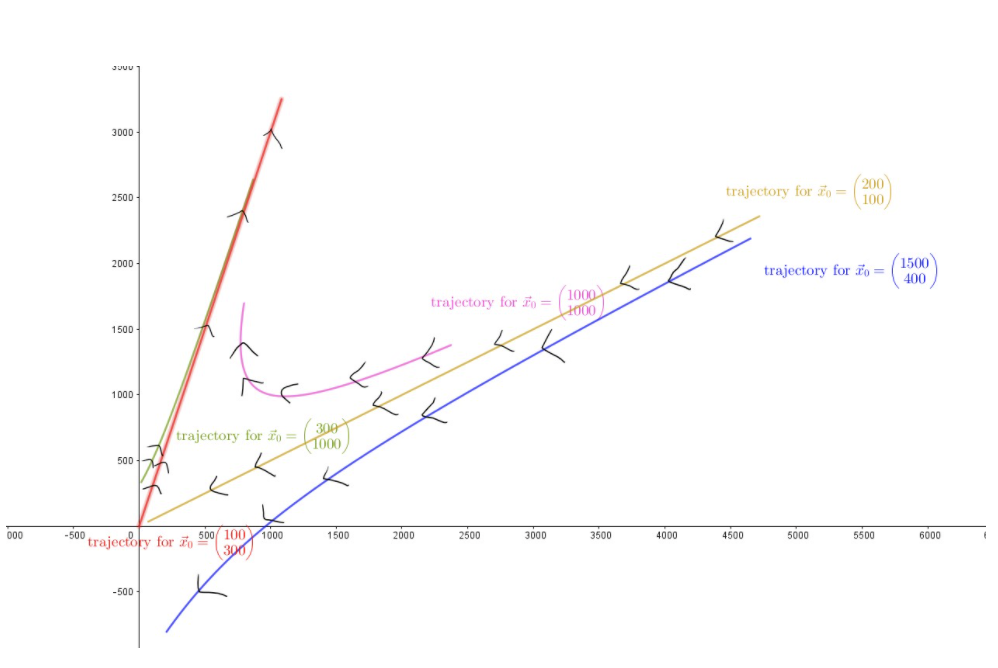
\includegraphics[scale=0.5]{state-vectors.png}
\end{center}

Called a \textbf{phase portrait} for a discrete dynamical system.
Indicates performing of system based on initial states.
The 2 state vectors in the basis are \textbf{eigenvectors}.

\begin{framed}
    If $A$ is an $n\times n$ matrix, an eigenvector of $A$ is a nonzero vector $\tb{v}$
    that has the property that $\tb{v}$ and $A\tb{v}$ are parallel.
    Same as saying that $A\tb{v}=\lambda\tb{v}$, so $\lambda$ is an eigenvalue.
\end{framed}

If there exists an $n\times n$ matrix $A$ with $\lambda=0$, then kernel of $A$ must be nontrivial
because $A\tb{v}=\tb{0}=0\tb{v}$, therefore $A$ is singular.